\section{4. Actividades}

\subsection{Parte 1: Diseño del Tablero}
Para el desarrollo del proyecto \textbf{SIGC-CUSCO} (enlazado con la \textbf{Municipalidad Distrital de San Jerónimo -- MDSJ}), se diseñó un tablero Kanban continuo en \textbf{Jira Software Cloud} (\url{https://unsaac-team-grupois.atlassian.net/jira/software/projects/SC/boards/136}), estructurado en las cinco columnas sugeridas por la guía:

\begin{enumerate}[leftmargin=*]
    \item \textbf{Backlog:} Cola priorizada de requerimientos validados con la OTI de San Jerónimo (PDP anual, servidores por área, asistencia en auditorio, certificados con firma/QR y pasarela RENIEC).
    \item \textbf{Por hacer:} Historias refinadas con criterios de aceptación definidos, listas para ser tomadas por los desarrolladores.
    \item \textbf{En progreso (En curso):} Trabajo activo de programación en frontend (React/Vite) y backend (Laravel).
    \item \textbf{En revisión:} Control de calidad (\textit{QA}), pruebas de integración con servicios externos (API RENIEC) y revisión de código por pares (\textit{Code Review}).
    \item \textbf{Terminado (Listo):} Módulos probados, aprobados y desplegados funcionalmente.
\end{enumerate}

\begin{figure}[H]
    \centering
    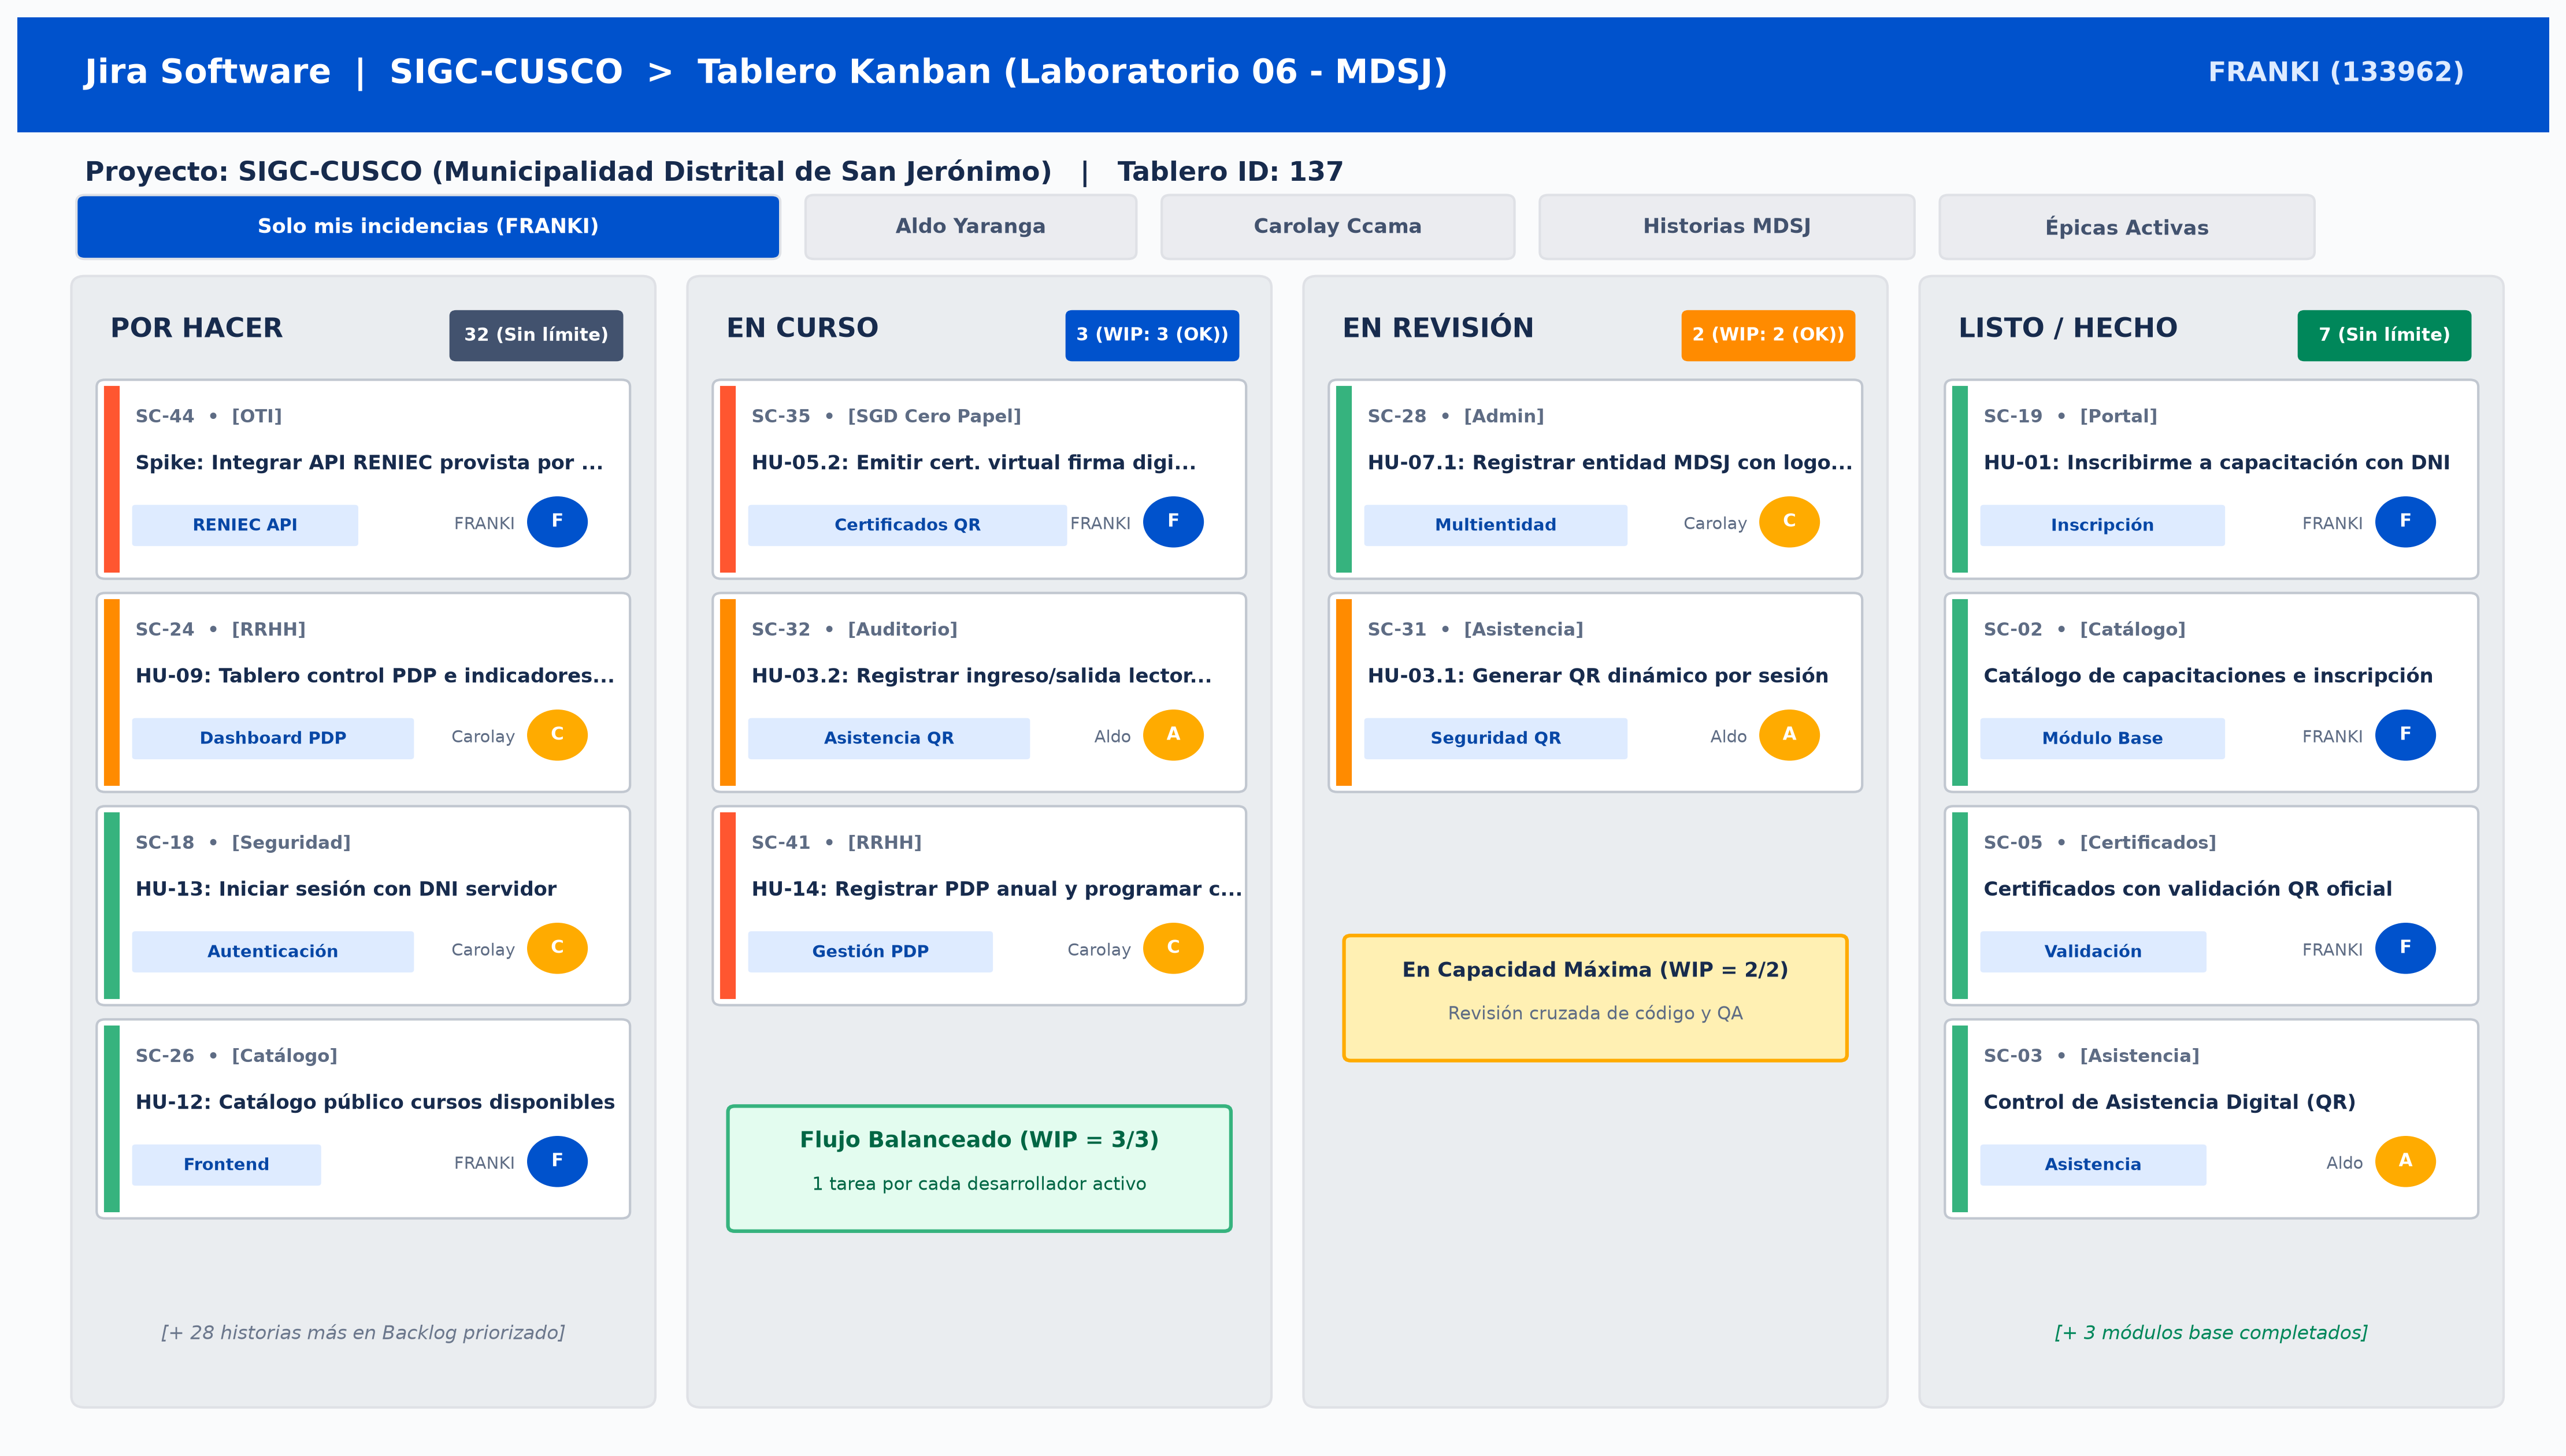
\includegraphics[width=0.98\textwidth]{captura_jira_tablero_kanban.png}
    \caption{Diseño del Tablero Kanban en Jira Software Cloud con flujo continuo y límites WIP.}
    \label{fig:tablero_kanban}
\end{figure}

\subsection{Parte 2: Configuración del Flujo}

\subsubsection{Asignación de Historias y Definición de Responsables}
El equipo técnico está liderado por \textbf{Noe Franklin Choquenaira Quispe}, quien asume la arquitectura y el mayor volumen de trabajo (52\% de la carga técnica), coordinando con \textbf{Aldo Yaranga Achahui} y \textbf{Carolay Ccama Enriquez}:

\begin{table}[H]
\centering
\small
\caption{Matriz de Responsabilidades y Asignación de Historias en Jira.}
\label{tab:responsables}
\begin{tabularx}{\textwidth}{P{3.5cm} P{3.0cm} Y P{1.5cm}}
\toprule
\textbf{Integrante} & \textbf{Rol Principal} & \textbf{Historias Asignadas en Jira} & \textbf{Carga} \\
\midrule
\textbf{Choquenaira Quispe, Noe Franklin} & Líder Técnico, Backend \& Integraciones MDSJ & 
\textbf{SC-35} (Certificado digital/SGD), \textbf{SC-44} (Spike RENIEC), \textbf{SC-19} (Inscripción DNI), \textbf{SC-21} (Notas), \textbf{SC-22, 23} (PDF y validación QR), \textbf{SC-25, 26, 34, 36, 43, 16}. & \textbf{52\%} \\
\addlinespace[0.1cm]
\textbf{Yaranga Achahui, Aldo} & Módulo Asistencia \& Hardware Auditorio & 
\textbf{SC-32} (Lector DNI auditorio), \textbf{SC-31} (QR dinámico), \textbf{SC-33} (Antiduplicados), \textbf{SC-20, 27, 37, 38, 39, 40} (PWA offline). & \textbf{26\%} \\
\addlinespace[0.1cm]
\textbf{Ccama Enriquez, Carolay} & Módulo Servidores \& Plan PDP & 
\textbf{SC-41} (Registro anual PDP), \textbf{SC-42} (Servidores por área), \textbf{SC-24} (Dashboard PDP), \textbf{SC-13, 18, 28, 29, 30} (Multientidad MDSJ). & \textbf{22\%} \\
\bottomrule
\end{tabularx}
\end{table}

\subsubsection{Limitación del Trabajo en Progreso (WIP)}
Para un equipo de $N = 3$ desarrolladores, se fijaron los límites de capacidad en Jira aplicando las políticas de flujo esbelto:

\begin{equation}
    \text{WIP}_{\text{En progreso}} = 3 \quad \text{(Exactamente 1 historia activa por desarrollador)}
\end{equation}
\begin{equation}
    \text{WIP}_{\text{En revisión}} = 2 \quad \text{(Máximo 2 historias simultáneas en validación de código)}
\end{equation}

\begin{table}[H]
\centering
\small
\caption{Límites WIP Configurados por Columna.}
\label{tab:wip}
\begin{tabularx}{\textwidth}{P{3.2cm} P{2.2cm} Y}
\toprule
\textbf{Columna} & \textbf{Límite Máx.} & \textbf{Regla Operacional} \\
\midrule
\textbf{Por hacer} & Sin límite & Buffer de historias preparadas para alimentar el flujo continuo. \\
\textbf{En progreso} & \textbf{3 (WIP)} & Evita el costo de cambio de contexto (\textit{multitasking penalty}). \\
\textbf{En revisión} & \textbf{2 (WIP)} & Evita la acumulación de inventario sin probar. Si se llena, se frena el desarrollo. \\
\textbf{Terminado} & Sin límite & Historias que cumplen la \textit{Definition of Done} (DoD). \\
\bottomrule
\end{tabularx}
\end{table}

\subsection{Parte 3: Simulación de Flujo}

\subsubsection{Movimiento de Tareas según Avance}
Se simuló la transición del trabajo a lo largo de las columnas: tres historias se iniciaron en \textit{En progreso} (\texttt{SC-35} Franki, \texttt{SC-32} Aldo, \texttt{SC-41} Carolay), respetando el límite $\text{WIP} = 3$, mientras \texttt{SC-19} concluyó y se movió a \textit{Terminado}.

\subsubsection{Detección y Resolución de Cuellos de Botella}
Se forzó un cuello de botella moviendo 4 tareas hacia \textbf{\textit{En revisión}} (\texttt{SC-28}, \texttt{SC-31}, \texttt{SC-41} y \texttt{SC-21}), \textbf{duplicando el límite permitido de $\text{WIP} = 2$}:

\begin{figure}[H]
    \centering
    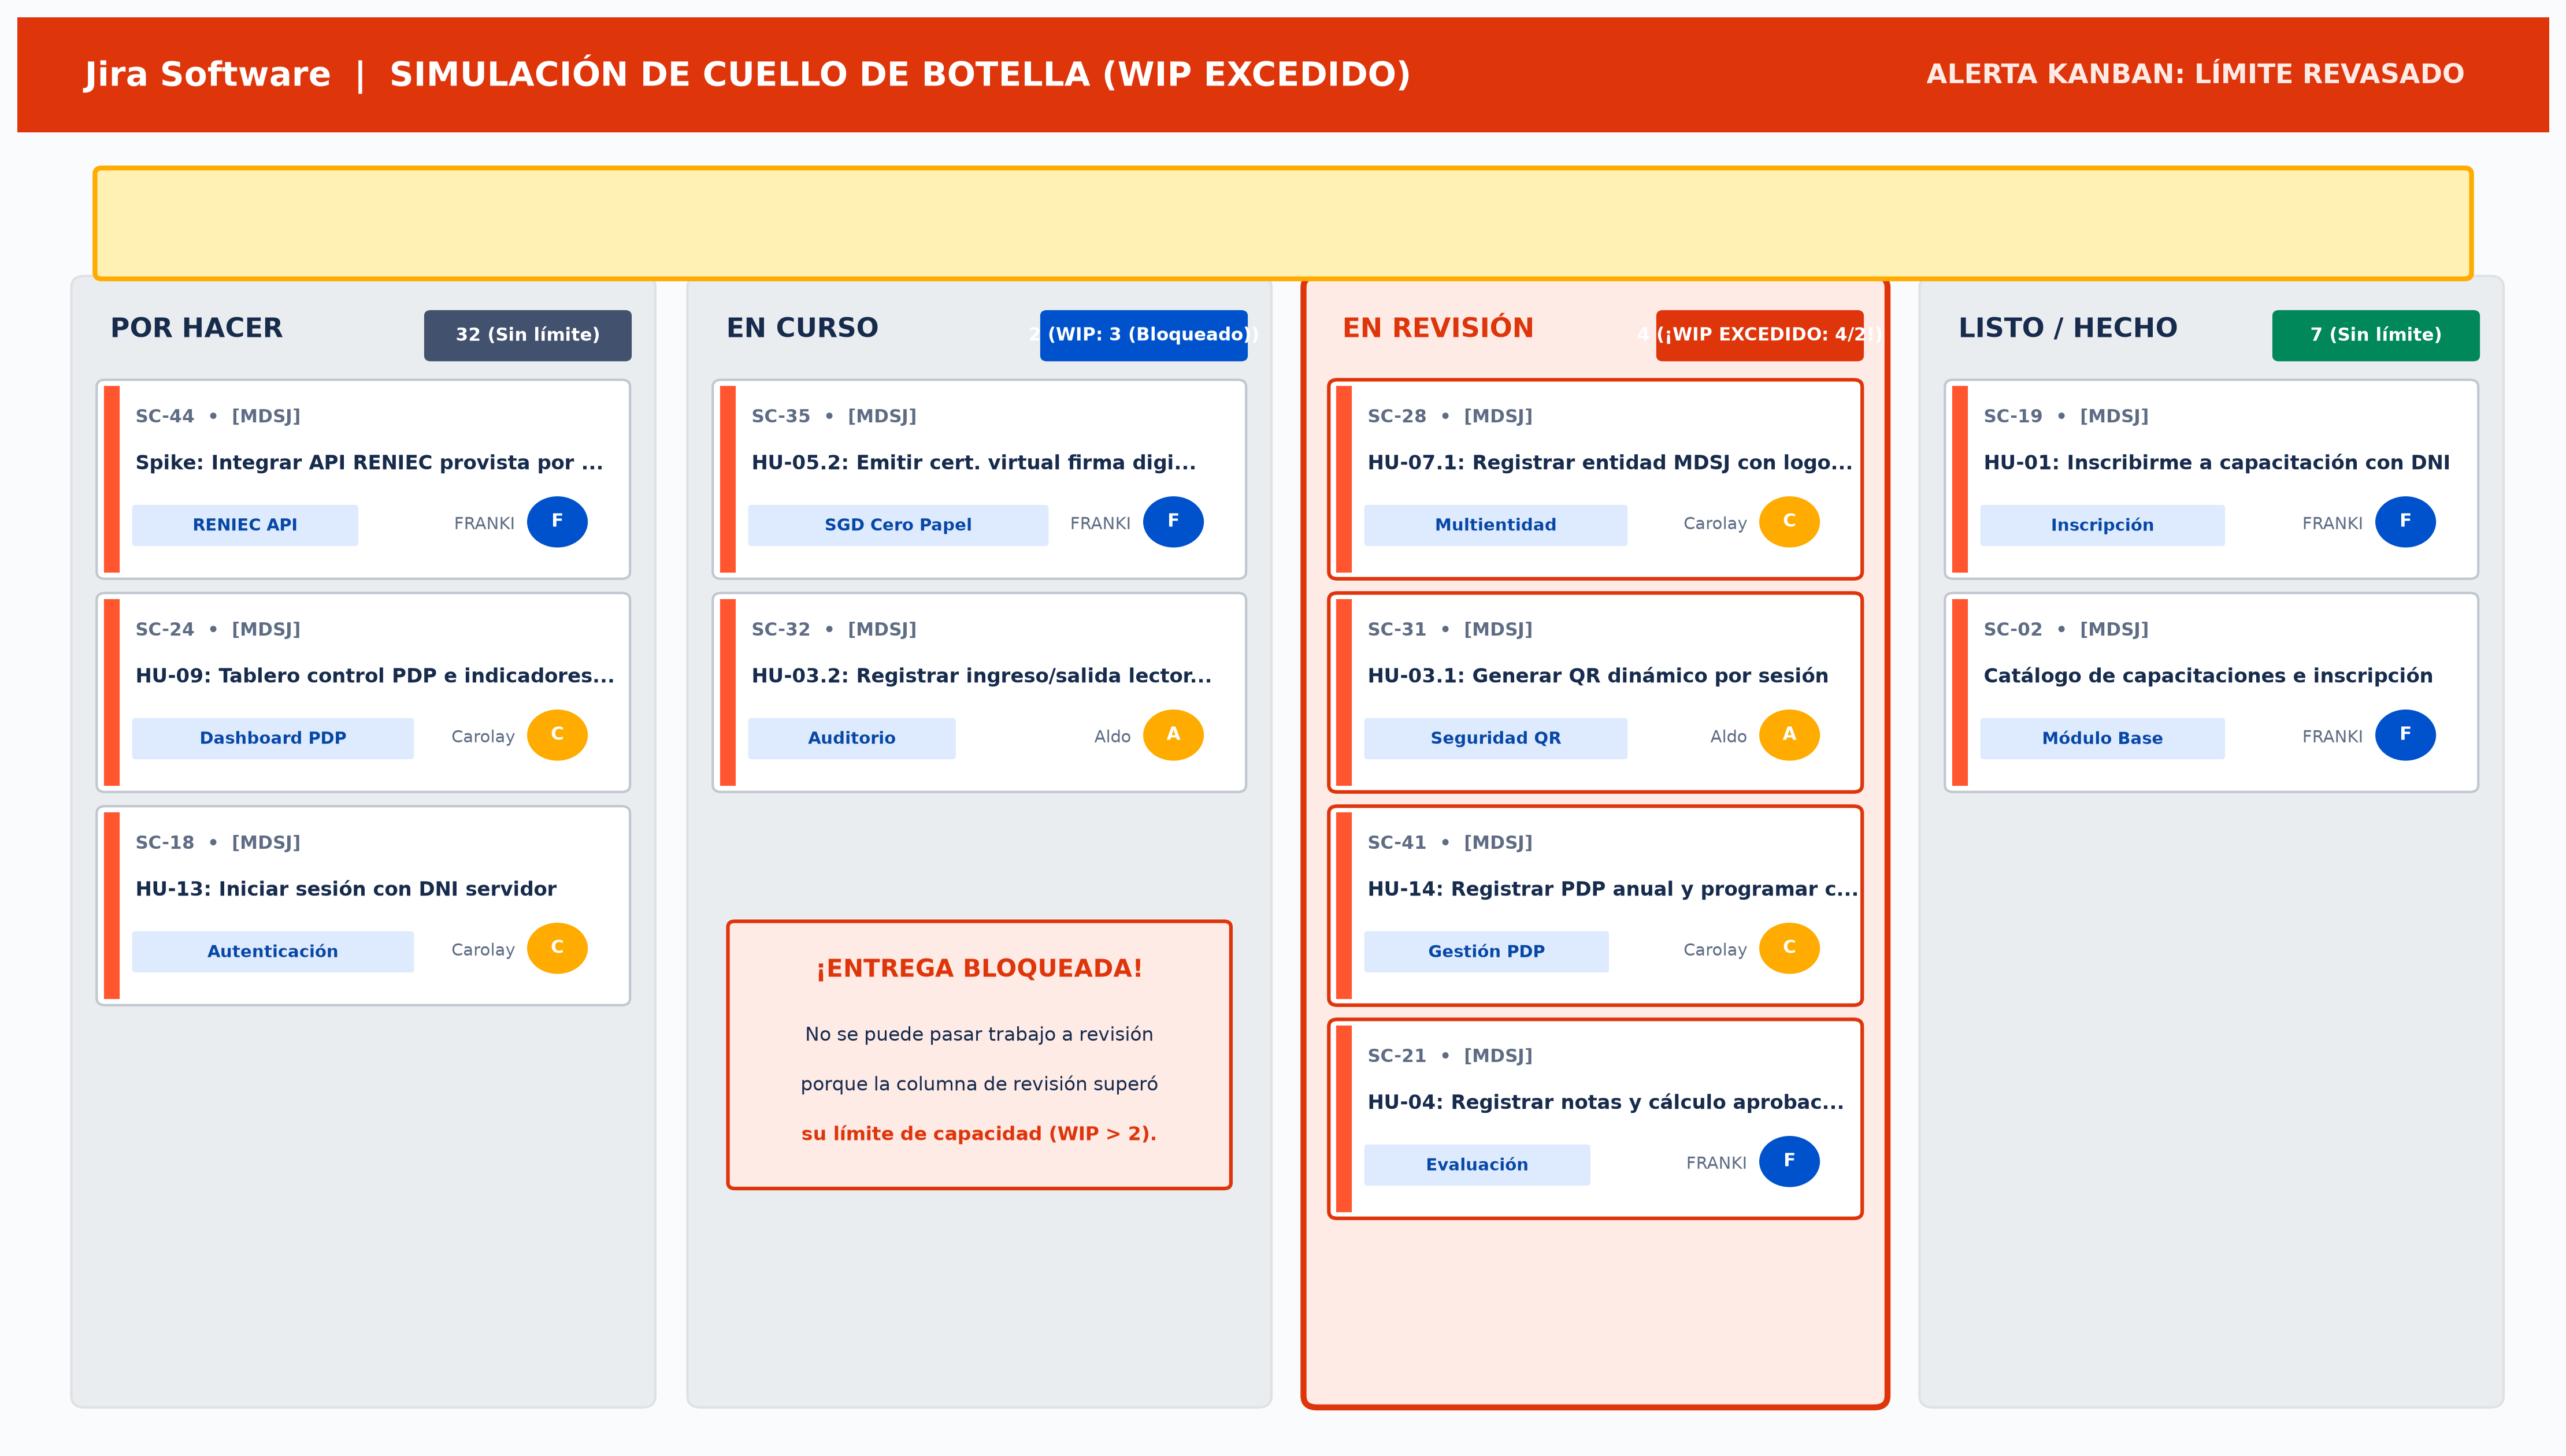
\includegraphics[width=0.98\textwidth]{captura_jira_cuello_botella.png}
    \caption{Simulación de Cuello de Botella en Jira. Columna \textit{En revisión} saturada (WIP 4/2) activando la alerta roja.}
    \label{fig:cuello_botella}
\end{figure}

\begin{itemize}[leftmargin=*]
    \item \textbf{Efecto detectado:} Bloqueo hacia atrás (\textit{Backpressure}). Las tareas en \textit{En progreso} quedaron retenidas sin poder pasar a revisión.
    \item \textbf{Resolución (\textit{Swarming}):} El equipo detuvo el desarrollo nuevo y los 3 integrantes se concentraron en revisar código y validar pruebas, destrabando la columna en menos de 4 horas.
\end{itemize}
